\documentclass[14pt]{extarticle}

\begin{document}
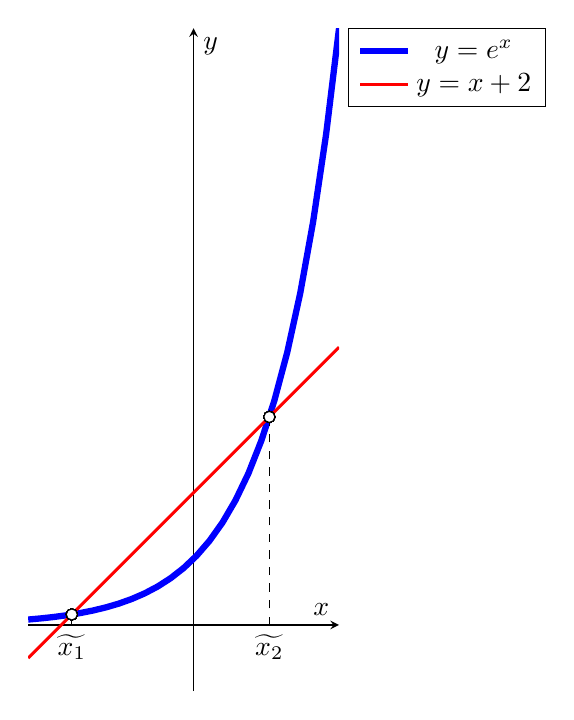
\begin{tikzpicture} [
	declare function = {
		g(\x)=e^\x;
		h(\x)=\x+2;
	},]

	\begin{axis} [
		unit vector ratio*=1 1,
		height=10cm,
		xlabel = {$x$},
		ylabel = {$y$},
		axis x line = middle,
		axis y line = middle,
		domain = -2.5:2.2,
		ymin = -1,
		ticks = none,
		legend pos = outer north east]

		\newcommand*{\Xfirst}{-1.841}
		\newcommand*{\Xsecond}{1.146}
		\pgfmathsetmacro{\fXfirst}{h(\Xfirst)}
		\pgfmathsetmacro{\fXsecond}{h(\Xsecond)}

		\addplot[color=blue, line width=.08cm]{g(x)};
		\addplot[color=red, line width=.04cm]{h(x)};

		\coordinate(X1) at 	(\Xfirst,	\fXfirst);
		\node[below](X1p) at 	(\Xfirst,	0)
			{$\widetilde{x_1}$};
		\coordinate(X2) at 	(\Xsecond,	\fXsecond);
		\node[below](X2p) at 	(\Xsecond,	0)
			{$\widetilde{x_2}$};

		\addplot[mark=*,only marks, fill=white]
			(\Xfirst,\fXfirst) node[above, pos=1]{};
		\addplot[mark=*,only marks, fill=white]
			(\Xsecond,\fXsecond) node[above, pos=1]{};

		\draw[dashed] (X1p) -- (X1)	(X2p) -- (X2);

		\addlegendentry{$y=e^x$};
		\addlegendentry{$y=x+2$};
	\end{axis}
\end{tikzpicture}
\end{document}
